% Qual o problema? porque é bom ter geração procedural terrenos
\section{Introdução}

\begin{frame}{Contextualização}
  \begin{itemize}
        \item Criar conteúdo para jogos manualmente exige muito esforço de trabalho
        \item Quanto maior o mundo virtual, tecnicamente mais tempo os jogadores irão explorar \cite{bevilacqua2009ferramenta}
    \end{itemize}
\end{frame}

\begin{frame}{Contextualização}
  \begin{figure}
		\centering
        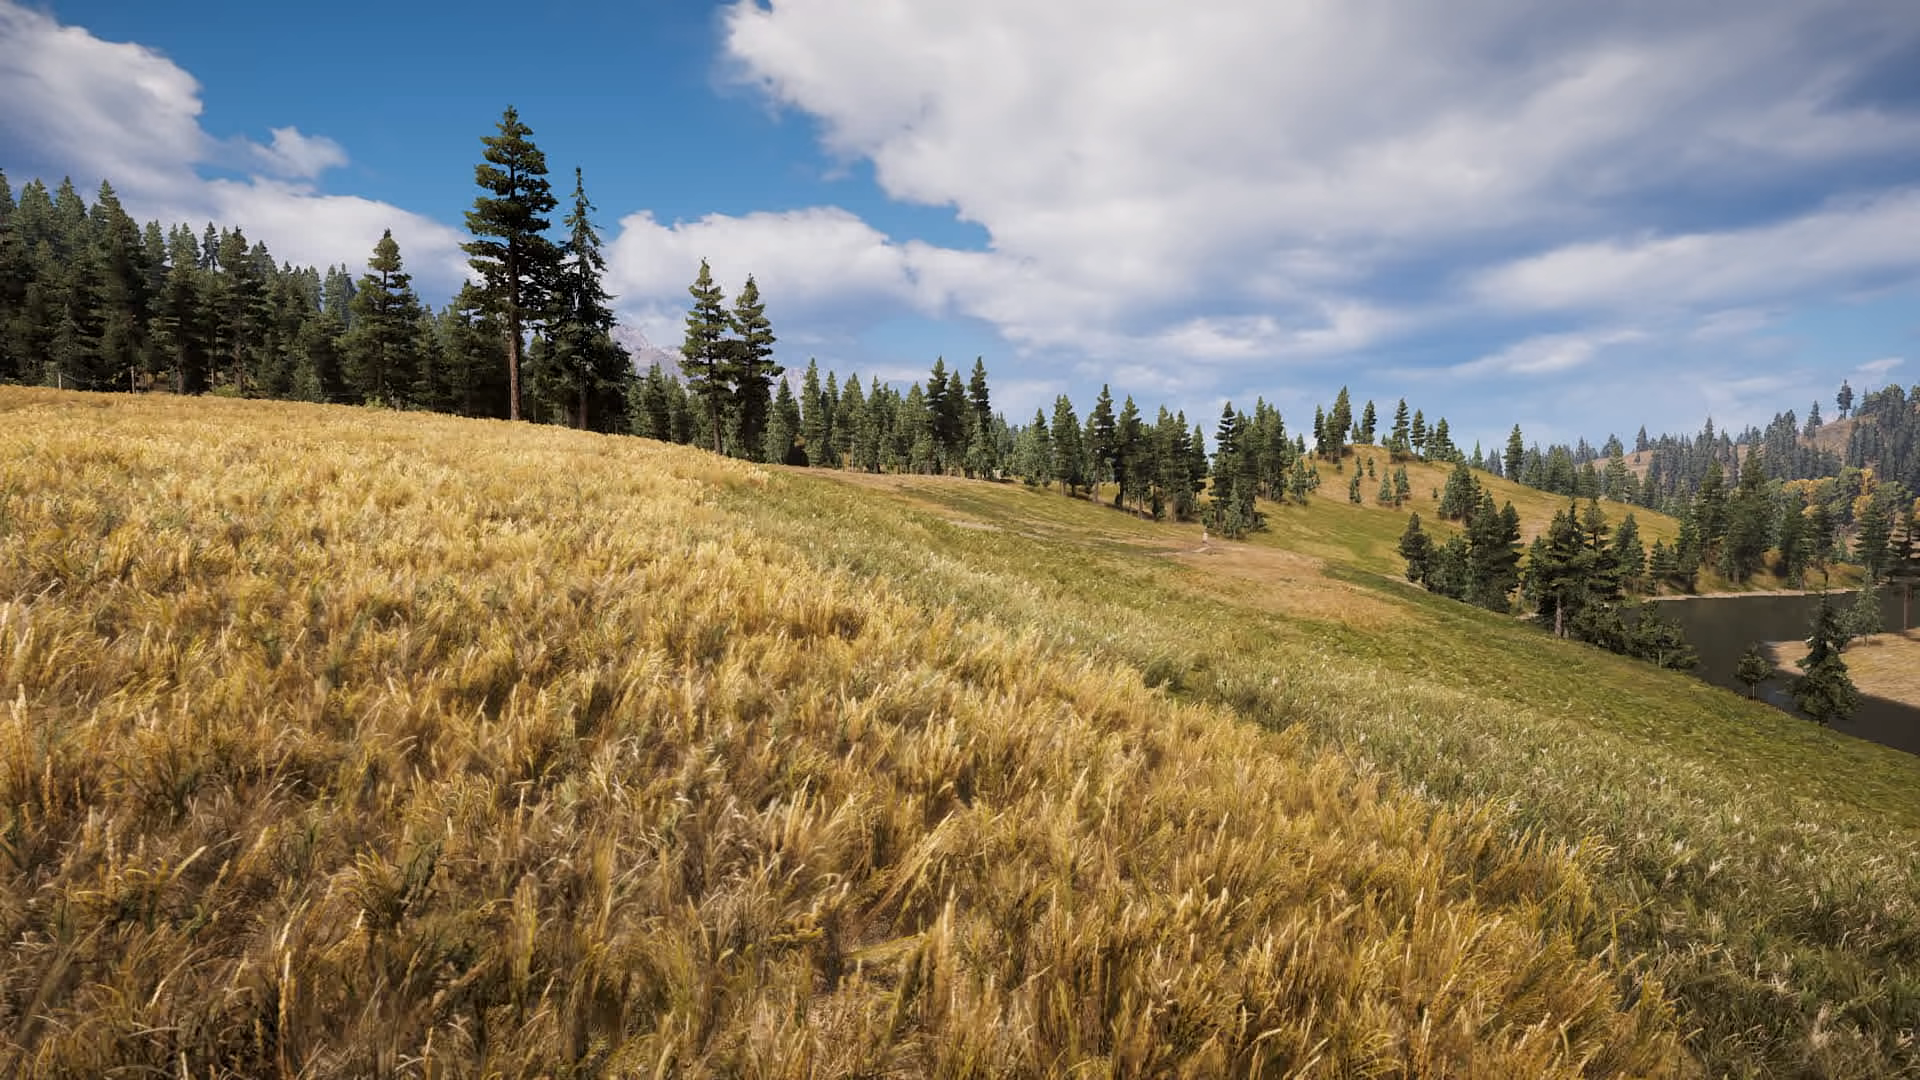
\includegraphics[width=.8\textwidth]{img/intro/fc5terrain.png}
        \caption{Mapa de \alert{Far Cry 5}, \cite{Carrier2018farcry5}}
  \end{figure}
\end{frame}